\chapter{Overview}
\label{sec:design_overview}
As part of a greater platform, the launcher is required to provide services to other components of the \giraf[] system, and may also depend on others.
\todo{HUSK, introducere de requirements som vi selv har sat for os selv}
The required services and dependencies are outlined below.

\autoref{fig:external_architecture} illustrates the \giraf[] launcher component. The component provides one service and have one dependency.
The services it provides is based on demands from the surrounding components of the \giraf[] platform, which can be seen in \autoref{fig:Giraf_comp_pic}.
The illustrated service provides a way for launched \girafapp[]s to determine which guardian launched the app in question, with which child profile, together with color data of the specific app.
The illustrated dependency represents the need for being able to read and update profile data. The service which fulfill this dependency is provided by the Oasis lib. 

As seen on \autoref{fig:Giraf_comp_pic}, Oasis is available for the launcher to use. Oasis stores the modulated data, including the guardian and child profiles on the device in a local database.


\begin{figure}[h]
	\centering
	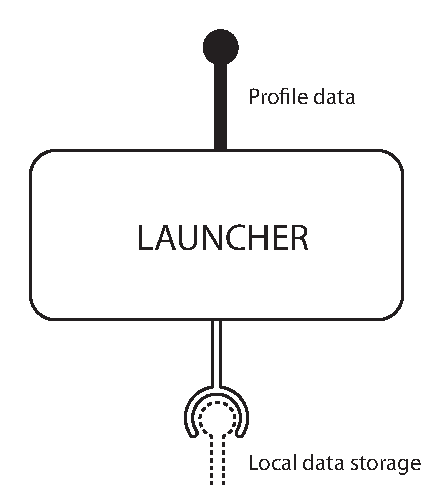
\includegraphics[width=0.5\textwidth]{gfx/external_launcher_architecture.pdf}
	\caption{The  \giraf[] launcher component.}
	\label{fig:external_architecture}
\end{figure}


Being able to launch an \girafapp[] as a specific guardian requires the user to interact such that the launcher knows which guardian the user represents.

Authentication was chosen, as each modulated child and guardian contains private data and therefore needs to be protected.

%This section presents an overview of the design work done on the overall product, and the following sections present details on specific features in the launcher. \newline

%The design of the \giraf[] launcher is centered around high usability and specific functionality requirements. 
%These functionality requirements come from both the customers of the project, and other \localgroup[]s in the multi project, and include only the requirements that are within the scope of this project. \newline


%The requirements are as follows:
%\begin{itemize}
%\item Allow \guardian[]s to launch apps.
%\item Allow each \guardian[] to customize their experience with the launcher. 
%\item Allow apps to work for a specific \autist[].
%\end{itemize}

%High usability has been prioritized, both because it was requested by the customer, but also because the launcher is planned to be expanded and usable by \autists[] later on.
%See \autoref{Preanalysis:Usability_for_children} for more information on the usability requirements of children. \newline

%The above requirements have resulted in an overall interaction design, which can be seen in \autoref{fig:state_diagram}, in the form of a state diagram.

\autoref{fig:state_diagram} shows all possible states and transitions, which the launcher can be in.
The states of the state diagram represent four functionalities of the launcher:

\begin{enumerate}
	\item Initialization
	\item Authentication
	\item App selection
	\item Profile selection
\end{enumerate}

These functionalities are shown in \autoref{fig:design_diagram}, along with the states of which they represent, and the transitions between them.

\begin{figure}[h]
	\centering
	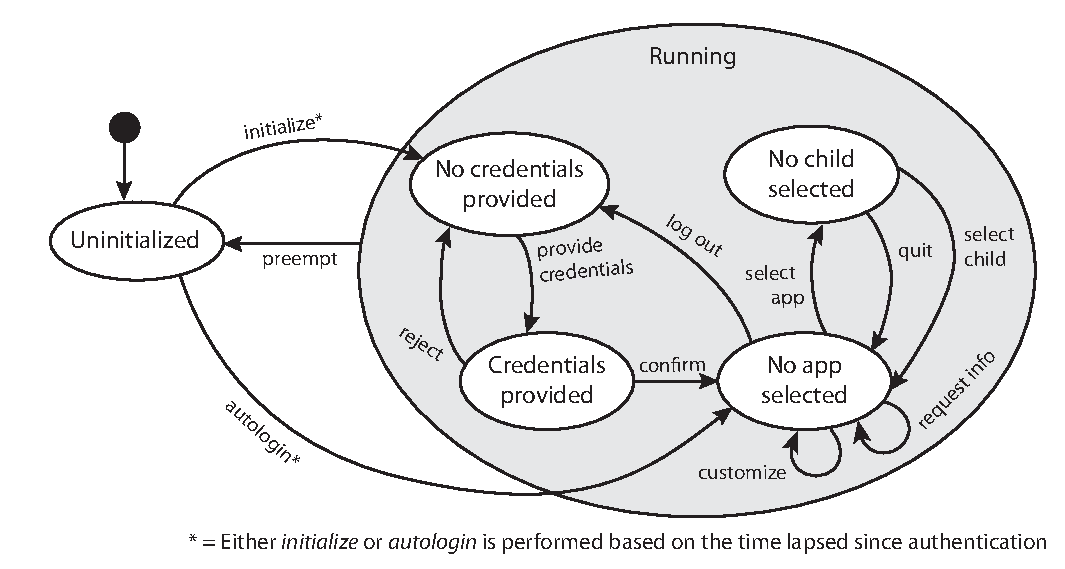
\includegraphics[width=1\textwidth]{gfx/statediagram.pdf}
	\caption{State diagram}
	\label{fig:state_diagram}
\end{figure}

%To make the design easier to approach, the system is split into four distinct features: Authentication, app management, profile selection, and resumption. 
%This split is illustrated in \autoref{fig:design_diagram}, which groups the states and actions of \autoref{fig:state_diagram} according to their to the feature they belong to. 

\begin{figure}[h]
	\centering
	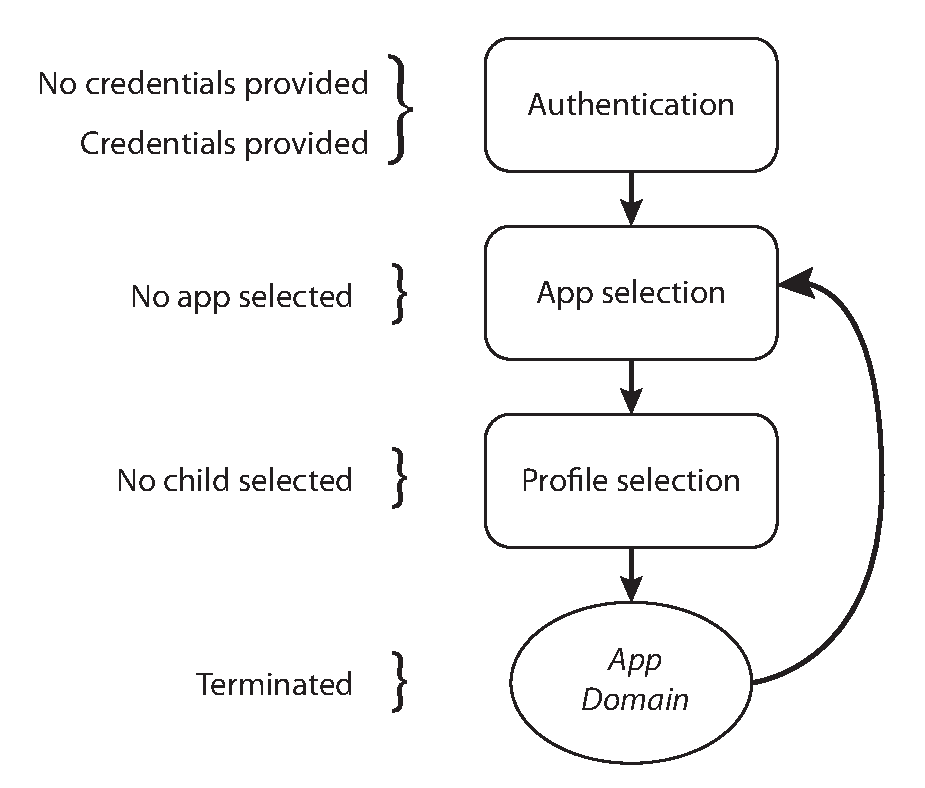
\includegraphics[width=1\textwidth]{gfx/design_diagram.pdf}
	\caption{Functionality diagram}
	\label{fig:design_diagram}
\end{figure}